\section{Assignments}\label{sec:assignments}

Assignments bezeichnen ein Feature von fulib.org, das sich mit dem Anlegen, Lösen und Bewerten von Hausaufgabenblättern sowie Online-Kursen beschäftigt.
Es handelt sich dabei um Modellierungsaufgaben in der Scenario-Sprache.
Diese können automatisch geprüft und manuell bewertet werden.
Der Unterabschnitt~\ref{subsec-creation} befasst sich zunächst mit dem Anlegen der Assignments aus Sicht des Kursleiters.
Daraufhin wird unter~\ref{subsec:solution} die Sicht der Studierenden bei der Lösung erläutert.
Auch des Vorgehen der Korrekteure zum Bewerten der Lösungen wird hier erläutert.
Zuletzt wird die Kurs-Funktion unter~\ref{subsec:courses} vorgestellt.

\subsection{Anlegen}\label{subsec:creation}

Das Anlegen von Assignments ist mit dem in Abbildung~\ref{fig:create-assignment} gezeigten Formular möglich.
Dafür muss lediglich im stets sichtbaren Seitenfooter unter ``Assignments'' der Menüeintrag ``Create Assignment'' ausgefählt werden.

% TODO größer, evtl. geteilt; mit Beispieleingaben
\begin{figure}
    \centering
    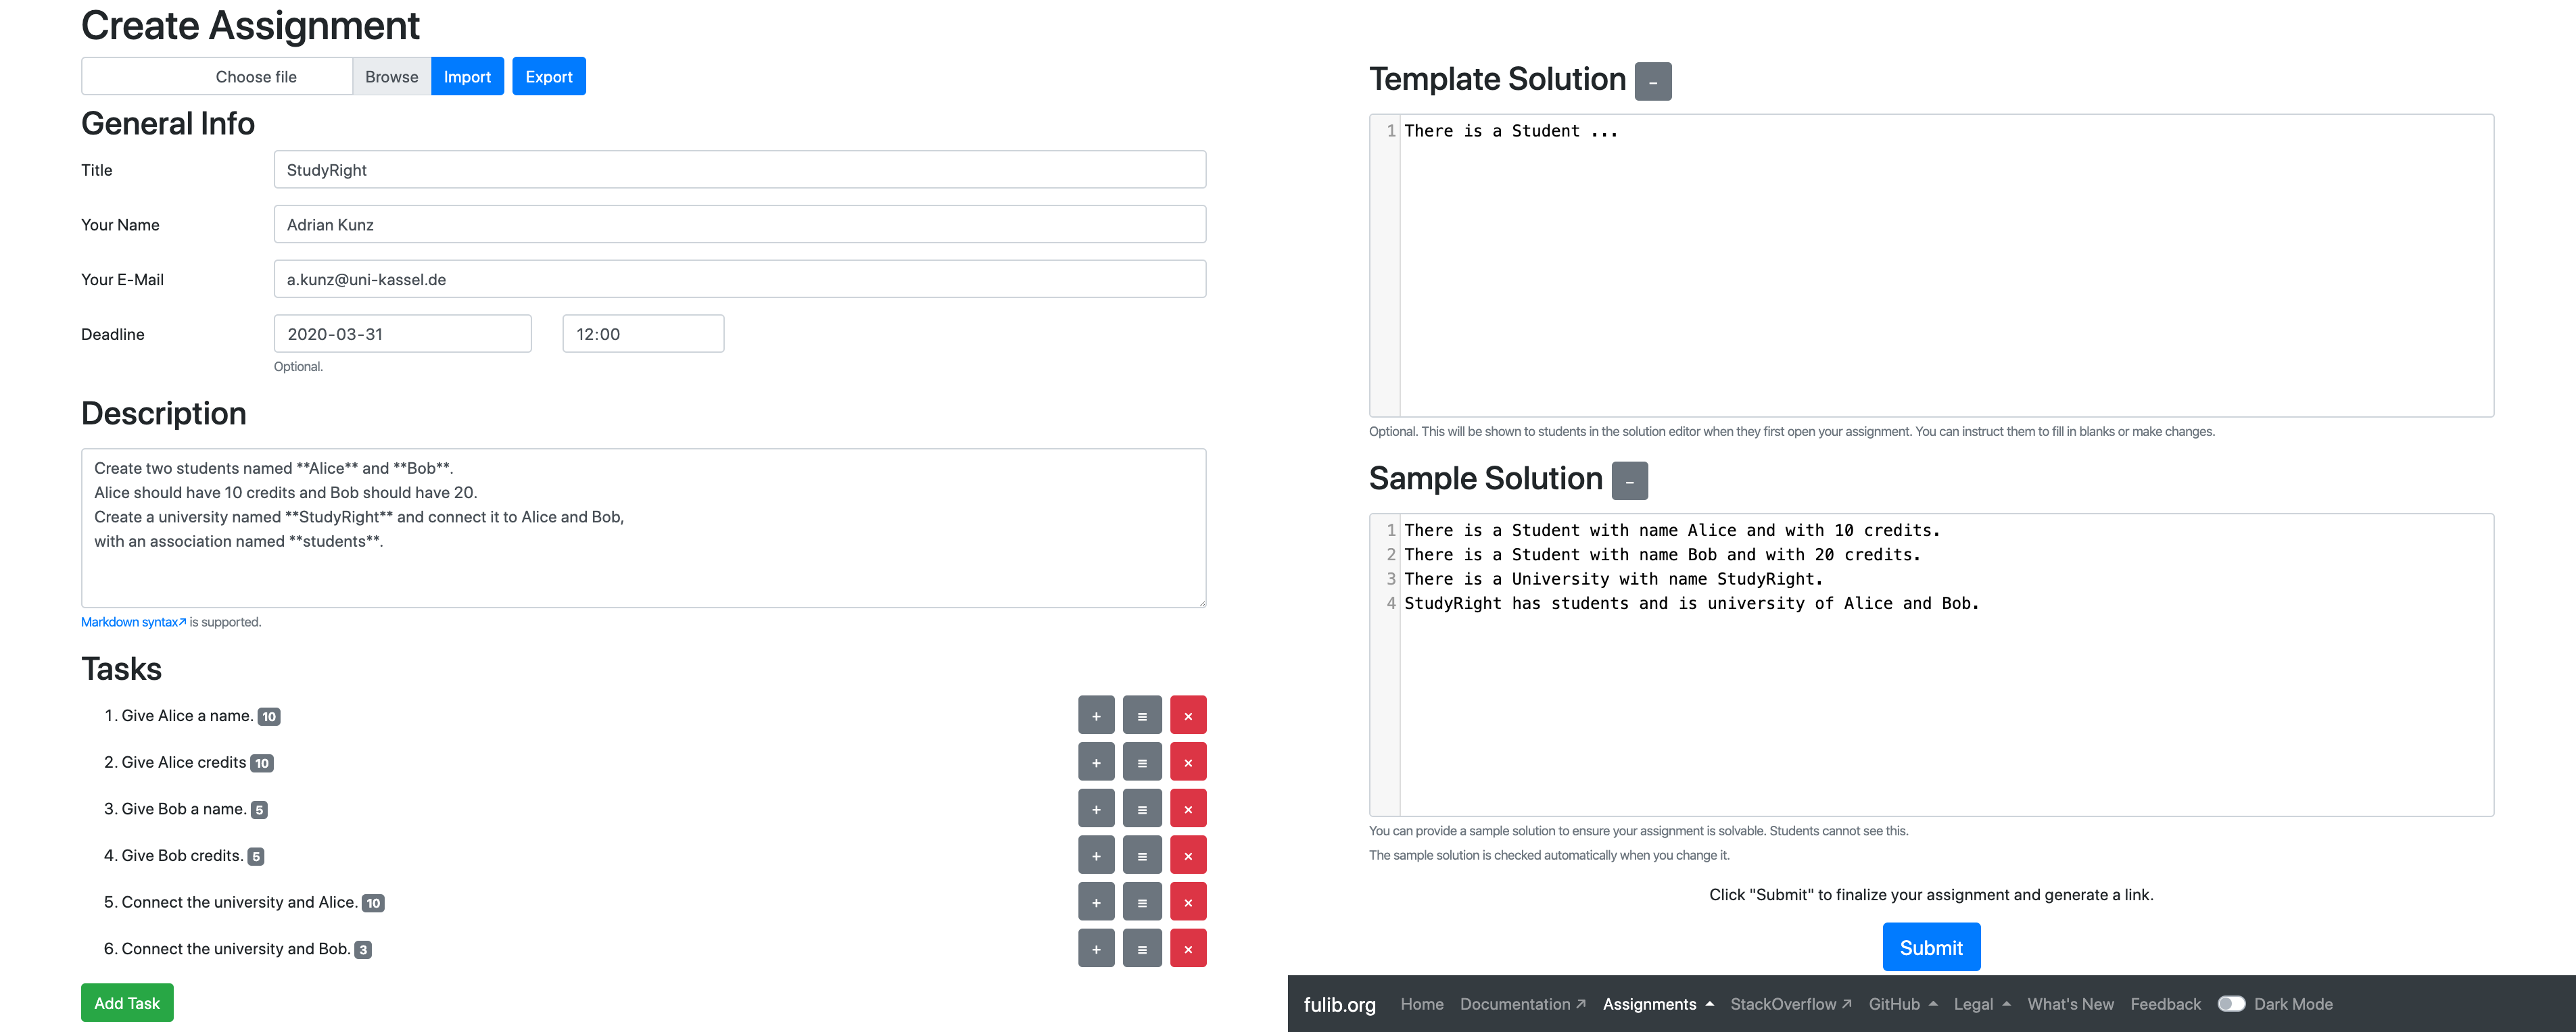
\includegraphics[width=0.5\textwidth]{chapter/fulib.org/img/create-assignment.png}
    \caption{Formular zum Anlegen von Assignments}
    \label{fig:create-assignment}
\end{figure}

Hier werden zunächst der Titel des Assignments sowie Name und E-Mail-Adresse des Kursleiters eingetragen.
Ebenso muss eine Deadline angegeben werden.
Das mit ``Description'' bezeichnete Feld ist für die Aufgabenstellung vorgesehen.
Dabei wird Markdown-Syntax unterstützt, es können also Überschriften, Tabellen, Listen, Bilder etc.\ eingebracht werden.

Als nächstes werden die Teilaufgaben (Tasks) eingetragen.
Mit dem Button ``Add Task'' kann der Liste ein neuer Task hinzugefügt werden.
Jeder Task hat eine kurze Beschreibung und eine maximal erreichbare Punktzahl.
Der mit ``Verification'' bezeichnete Editor ist dafür vorgesehen, einen Teil eines Scenarios mit Expect-Sätzen einzutragen.
Ein Task wird später wie folgt automatisch bewertet:
Zunächst wird das hier eingetragene Teilscenario an die Lösung des Studierenden angehängt.
Das entstehende Scenario wird dann kompiliert und die entstandenen Tests werden ausgeführt.
Erzeugt dies einen Compilerfehler und schlägt der Test fehl, gilt die Teilaufgabe als nicht bestanden und wird mit null Punkten bewertet.
Andernfalls wird die maximal erreichbare Punktzahl vergeben.

Dies lässt sich an einem einfachen Beispiel demonstrieren.
Angenommen, die Beschreibung eines Tasks lautet, dass ein Objekt \code{alice} mit dem Wert \code{Alice} in einem Attribut \code{name} erstellt werden soll.
Der zugehörige Verifikationscode könnte dies wie folgt prüfen:

\begin{mdcodeblock}
    We expect that alice has name 'Alice'.
\end{mdcodeblock}

Eine mögliche Lösung wäre dann folgender Satz:

\begin{mdcodeblock}
    There is a Student with name Alice.
\end{mdcodeblock}

Bei deren Prüfung wird diese automatisch mit dem Verifizierungscode in ein vollständiges Scenario verpackt:

\begin{mdcodeblock}
    # Scenario
    There is a Student with name Alice.
    ## Verification
    We expect that alice has name 'Alice'.
\end{mdcodeblock}

Wird dieses kompiliert und der entstehende JUnit-Test ausgeführt, ist dieser erfolgreich.
Folglich wird auf den Task die volle Punktzahl vergeben.
Andererseits entspricht die folgende Lösung nicht der Aufgabenstellung:

\begin{mdcodeblock}
    There is a Student with name Bob.
\end{mdcodeblock}

Fügt man diese wie oben mit dem Verifizierungscode zusammen und kompiliert das Result,
wird der Scenario-Compiler aufgrund der fehlenden Variable \code{alice} eine Fehlermeldung bei \code{alice has name ...} erzeugen.
Die Fehlermeldung wird als Nichterfüllen des Tasks aufgefasst,
wodurch er mit null Punkten bewertet wird.

Zur Übersichtlichkeit lassen sich die einzelnen Tasks mit dem ``+''- bzw.\ ``-''-Button ein- und ausklappen.
Mit der Schaltfläche rechts davon lassen sich Tasks durch Ziehen mit Maus bzw.\ Finger anordnen.
Der rote ``x''-Button löscht den Task aus der Liste.

Unter der Task-Liste befinden sich die Eingabefenster für die Lösungsvorlage (Template Solution) und die Musterlösung (Sample Solution).
Beide lassen sich mit den entsprechenden Buttons ein- und ausklappen, um das Formular übersichtlicher zu machen.
Gibt man eine Vorlage an, so wird diese den Studierenden als Lösung vorgegeben, wenn sie das Assignment öffnen.
Die Aufgabenstellung könnte dann beispielsweise sein, dass das vorgegebene Scenario angepasst oder vervollständigt wird.
Dafür könnten in der Vorlage z.B.\ Lücken mit ``\code{...}'' gelassen werden, die der Studierende ausfüllen soll.
Für das zuvor genannte Beispiel wäre etwa eine Vorlage wie \code{There is a ...} vorstellbar.

Die Musterlösung ist zwar optional, sie erlaubt jedoch dem Ersteller, seine Aufgabenstellung auf Lösbarkeit zu prüfen.
Dadurch können Fehler in der Aufgabenstellung oder der Verifizierung frühzeitig erkannt werden.
Bei Änderung der Musterlösung wird sie automatisch geprüft.
In der Task-Liste werden dann diejenigen Tasks rot, deren Verifizierung fehlgeschlagen ist.
Dies deutet an, dass es ein Problem entweder in der Musterlösung oder im Verifizierungscode eines Tasks gibt.

Sämtliche Änderungen am Formular werden sofort im Browser gespeichert.
Dadurch wird Datenverlust beim Verlassen der Seite oder bei Ausfall der Internetverbindung vermieden.
Dennoch gibt es die Möglichkeit, den Entwurf des Assignments als Datei auf der Festplatte zu speichern.
Dies ist mit dem ``Export''-Button möglich.
Später kann diese Datei dann wieder in das Formular übernommen werden.
Dafür muss diese im Feld neben dem ``Import''-Button ausgewählt werden und anschließend auf diesen geklickt werden.
Die Import/Export-Funktion erlaubt ferner, ein Assignment für die spätere Bearbeitung zu speichern und ein Neues zu erstellen.
Heruntergeladene Dateien können weiterhin über E-Mail oder Filesharing an andere weitergegeben werden,
die das Assignment dann importieren und prüfen oder verändern können.

Um ein fertiges Assignment zu veröffentlich, genügt ein Klick auf den ``Submit''-Button.
Dieser bewirkt, dass das ausgefüllte Formular an den Server gesendet wird, der das erstellte Assignment speichert und einen Link generiert.
Abbildung~\ref{fig:create-assignment-success} zeigt das Fenster, das sich daraufhin öffnet und diesen Link zeigt.

\begin{figure}
    \centering
    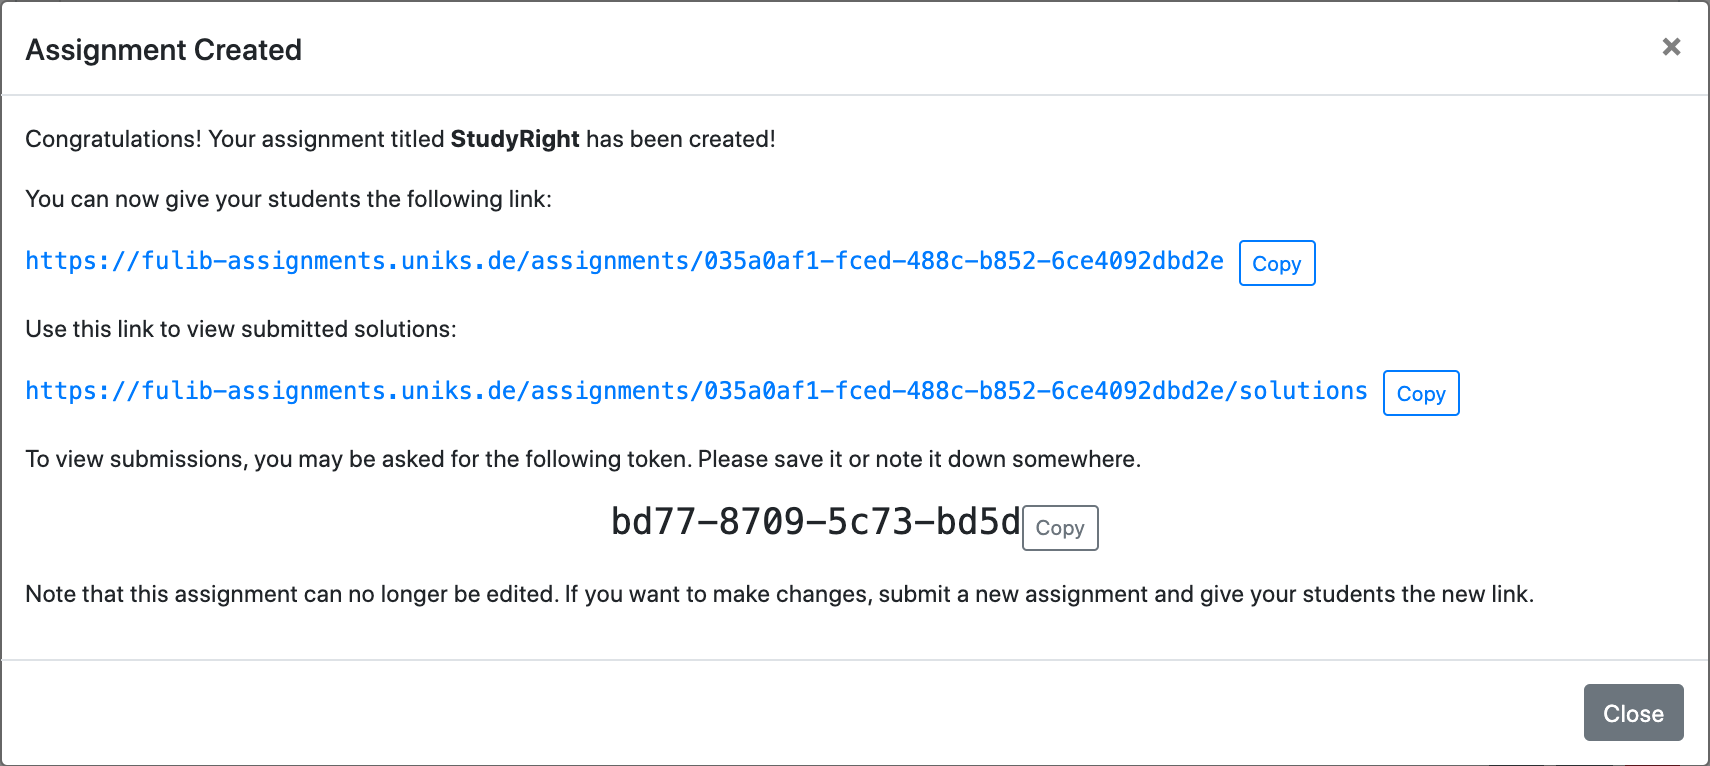
\includegraphics[width=\textwidth]{chapter/fulib.org/img/create-assignment-success.png}
    \caption{Fenster nach Anlegen eines Assignments}
    \label{fig:create-assignment-success}
\end{figure}

Der erste Link ist dafür vorgesehen, ihn an die Studierenden weiterzuleiten.
Öffnen sie diesen, zeigt sich die Seite, in der sie ihre Lösung des Assignments erstellen und abgeben können.
Dieser Vorgang ist Thema des nächsten Unterabschnitts.
Der zweite Link ist für den Kursleiter und die Korrekteure, da darunter eine Liste aller abgegeben Lösungen zu finden ist.
Um darauf zugreifen zu können, wird das gezeigte Token benötigt.
Dieses muss vom Kursleiter an die Korrekteure weitergeleitet werden.
Ohne dieses Token-System könnten Studierende die Lösungen von Anderen einsehen und übernehmen.

Assignments sind nach dem Einreichen nicht mehr veränderbar.
Dies ist gewünscht, da das Verändern von Assignments, die schon von Studierenden bearbeitet wurden, für diese nachteilhaft ist.
Wird im Nachhinein ein Fehler in der Aufgabenstellung erkannt, kann das gleiche Assignment erneut eingereicht werden.
Dabei werden neue Links und Token generiert, die wieder entsprechend geteilt werden müssen.

Wählt man im Footer Assignments \textrightarrow{} My Assignments aus, gelangt man zur Übersicht der eigenen Assignments.
Abbildung~\ref{fig:my-assignments} zeigt, wie diese Seite aussehen kann.

\begin{figure}
    \centering
    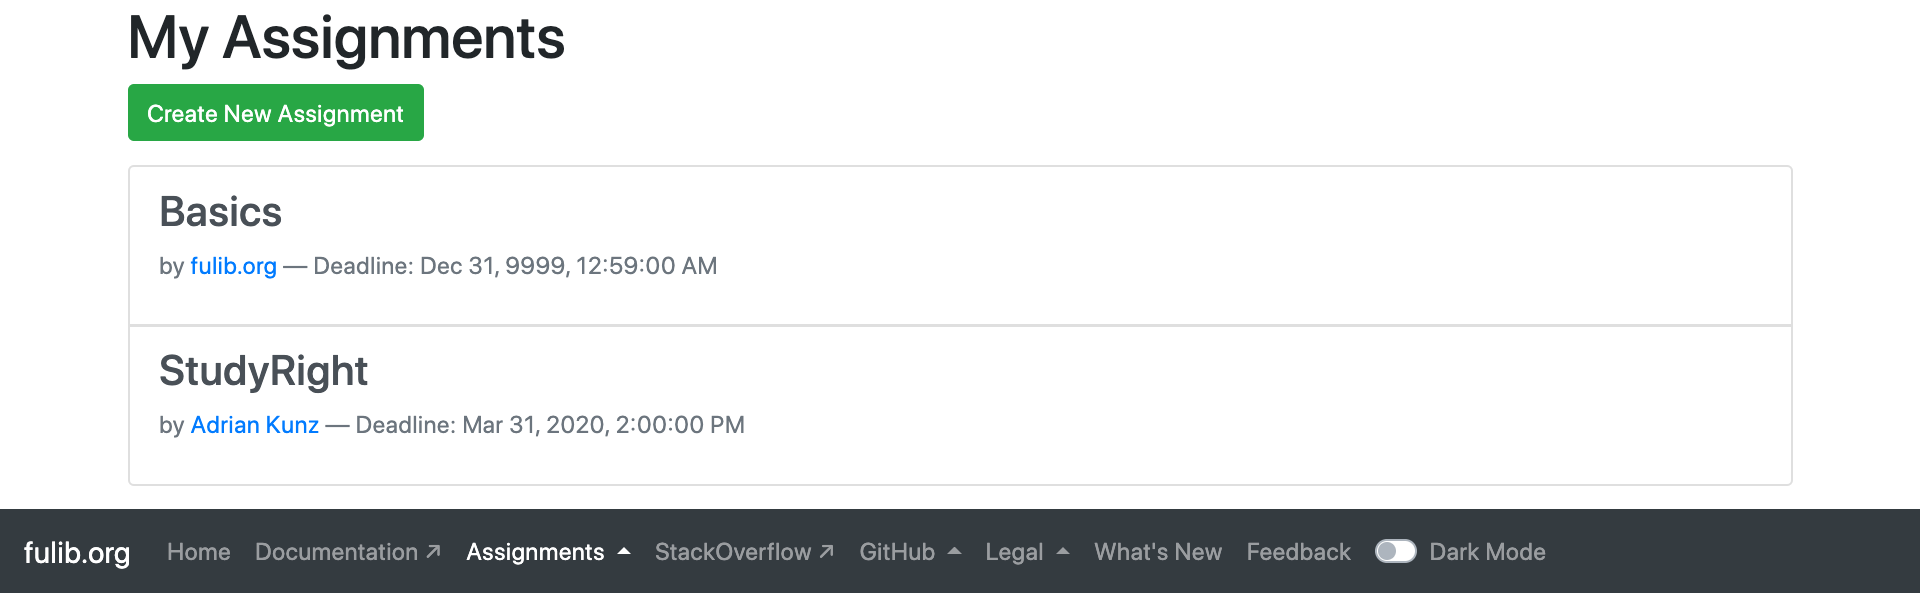
\includegraphics[width=\textwidth]{chapter/fulib.org/img/my-assignments.png}
    \caption{Liste der eigenen Assignments}
    \label{fig:my-assignments}
\end{figure}

Zu eigenen Assignments zählen die selbst erstellten sowie diejenigen, deren Token im Browser gespeichert ist.
Somit können auch Korrekteure hier die Assignments finden, die sie korrigieren sollen.
Für den Kursleiter kann diese Liste auch nützlich sein, wenn ein Link verloren gegangen ist.
Ein Klick auf einen Eintrag der Liste leitet auf die Liste mit Lösungen für das jeweilige Assignment weiter.

\subsection{Lösen}\label{subsec:solution}

Studierende können ein Assignment lösen, indem sie dessen Link besuchen.
Daraufhin wird die in Abbildung~\ref{fig:assignment-solve} gezeigte Seite angezeigt.
Diese enthält alle beim Erstellen angegebenen Eckdaten, sowie die Beschreibung und Task-Liste des Assignments.
Darunter befindet sich der Editor für die Lösung.
In Abbildung~\ref{fig:assignment-solve} enthält dieser bereits die vom Ersteller vorgegebene Lösungsvorlage als Hilfe zum Einstieg.

\begin{figure}
    \centering
    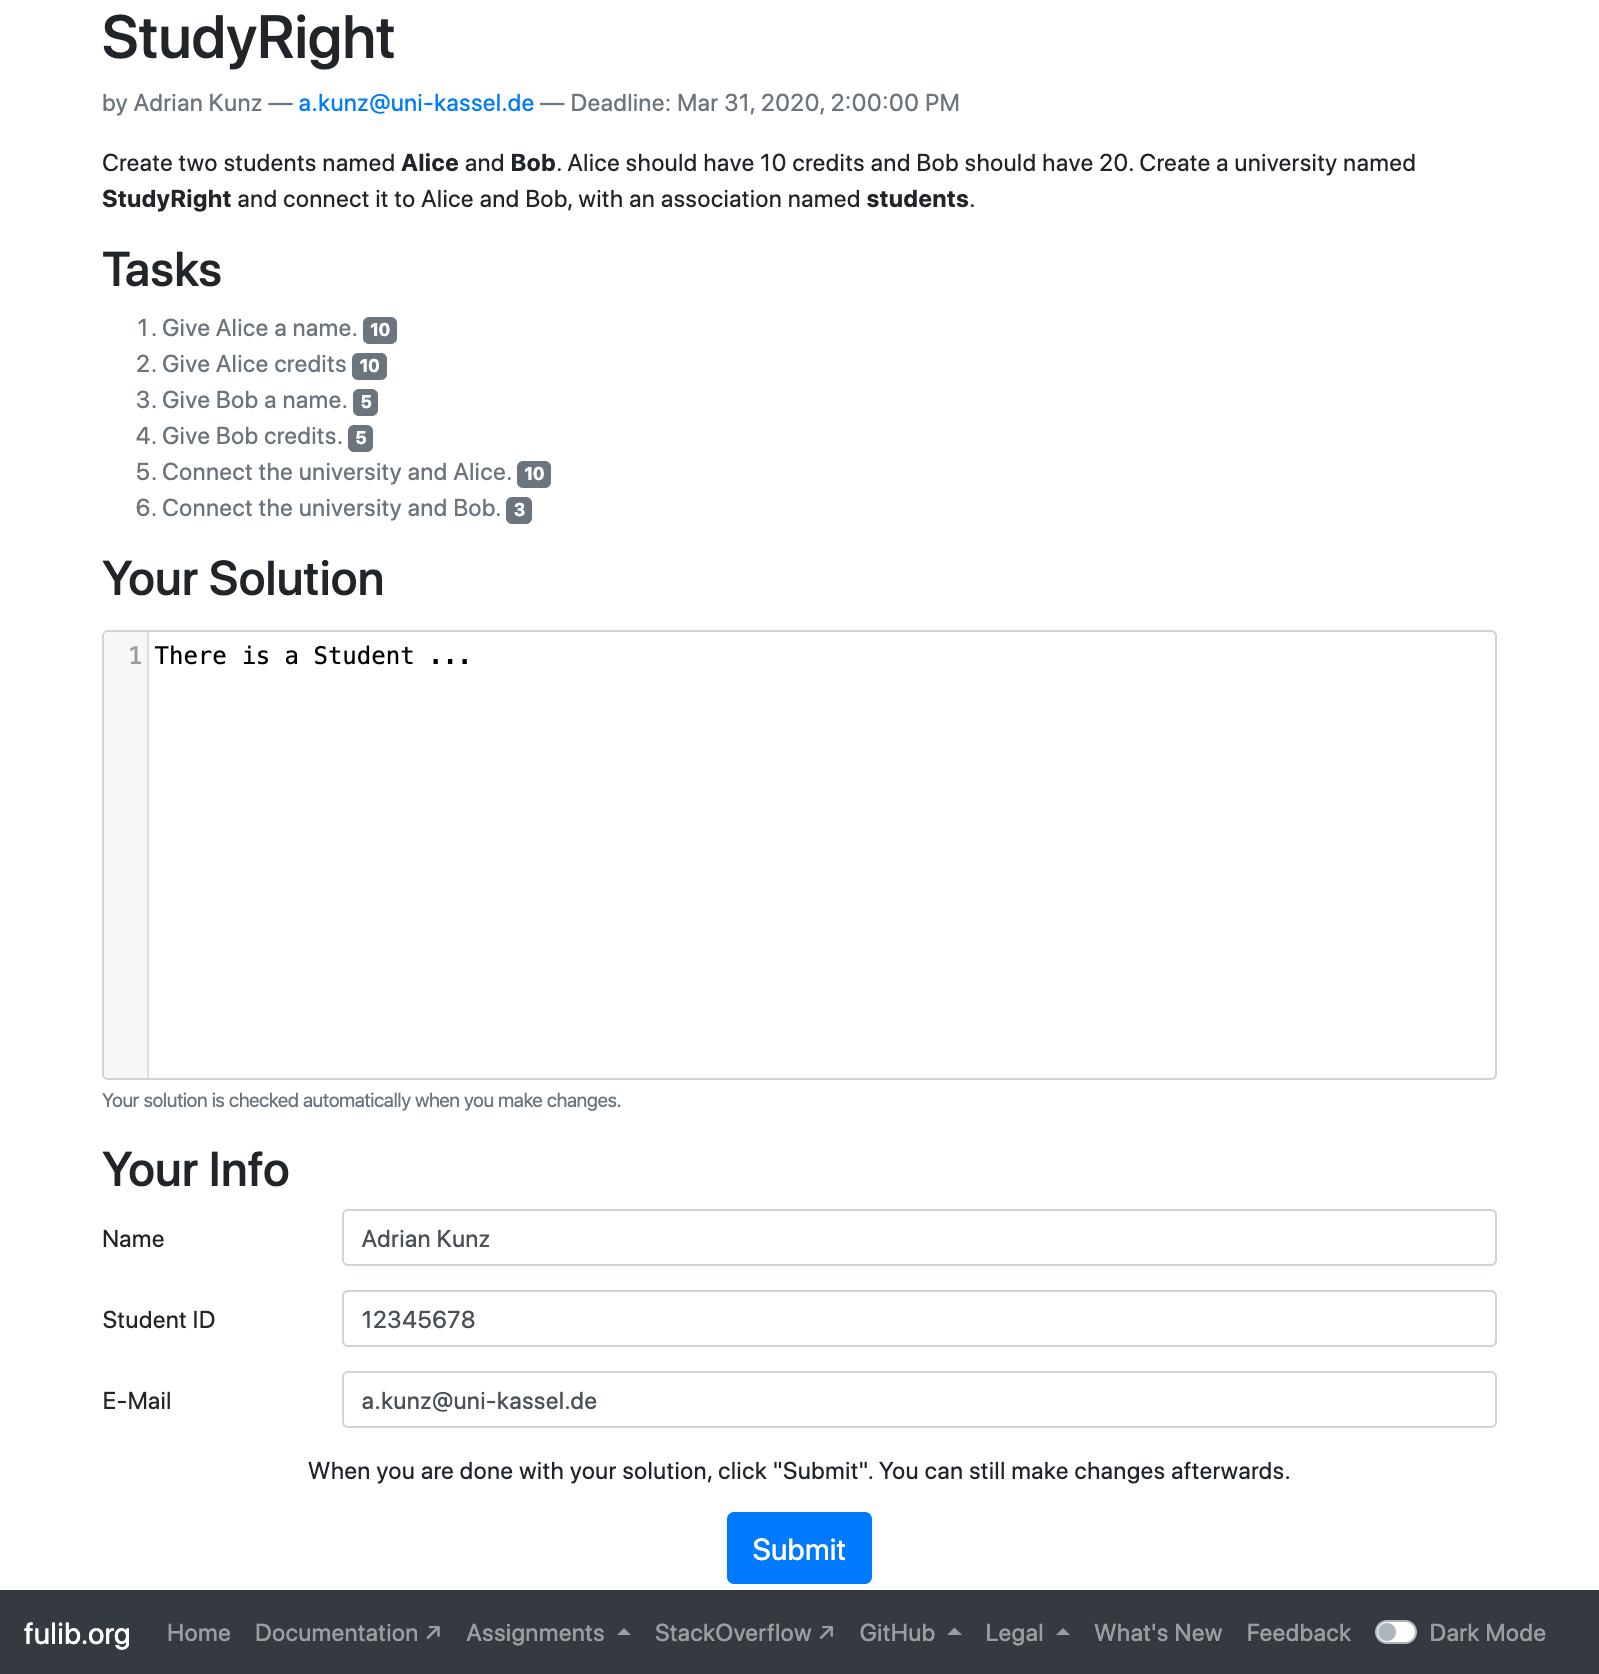
\includegraphics[width=\textwidth]{chapter/fulib.org/img/assignment-solve.png}
    \caption{Lösungsseite für ein Assignment}
    \label{fig:assignment-solve}
\end{figure}

Sobald man das Scenario im Editor bearbeitet, beginnt die automatische Prüfung anhand der Tasks.
Dabei werden erfüllte Tasks grün und nicht erfüllte Tasks rot.
Auch die erreichte Punktzahl wird ermittelt und angezeigt.
Bei nicht erfüllten Tasks lässt sich mit ``View Output'' die Ausgabe des Scenario-Compilers anzeigen, welche auf die Fehlerursache hinweist.
Abbildung~\ref{fig:solve-tasks} zeigt, wie dies bei einer Teillösung aussehen kann.
Der Studierende kann dann seine Lösung anpassen, um alle Tasks zu erfüllen.
Es ist jedoch auch möglich, eine (teilweise) fehlerhafte Lösung abzugeben.

\begin{figure}
    \centering
    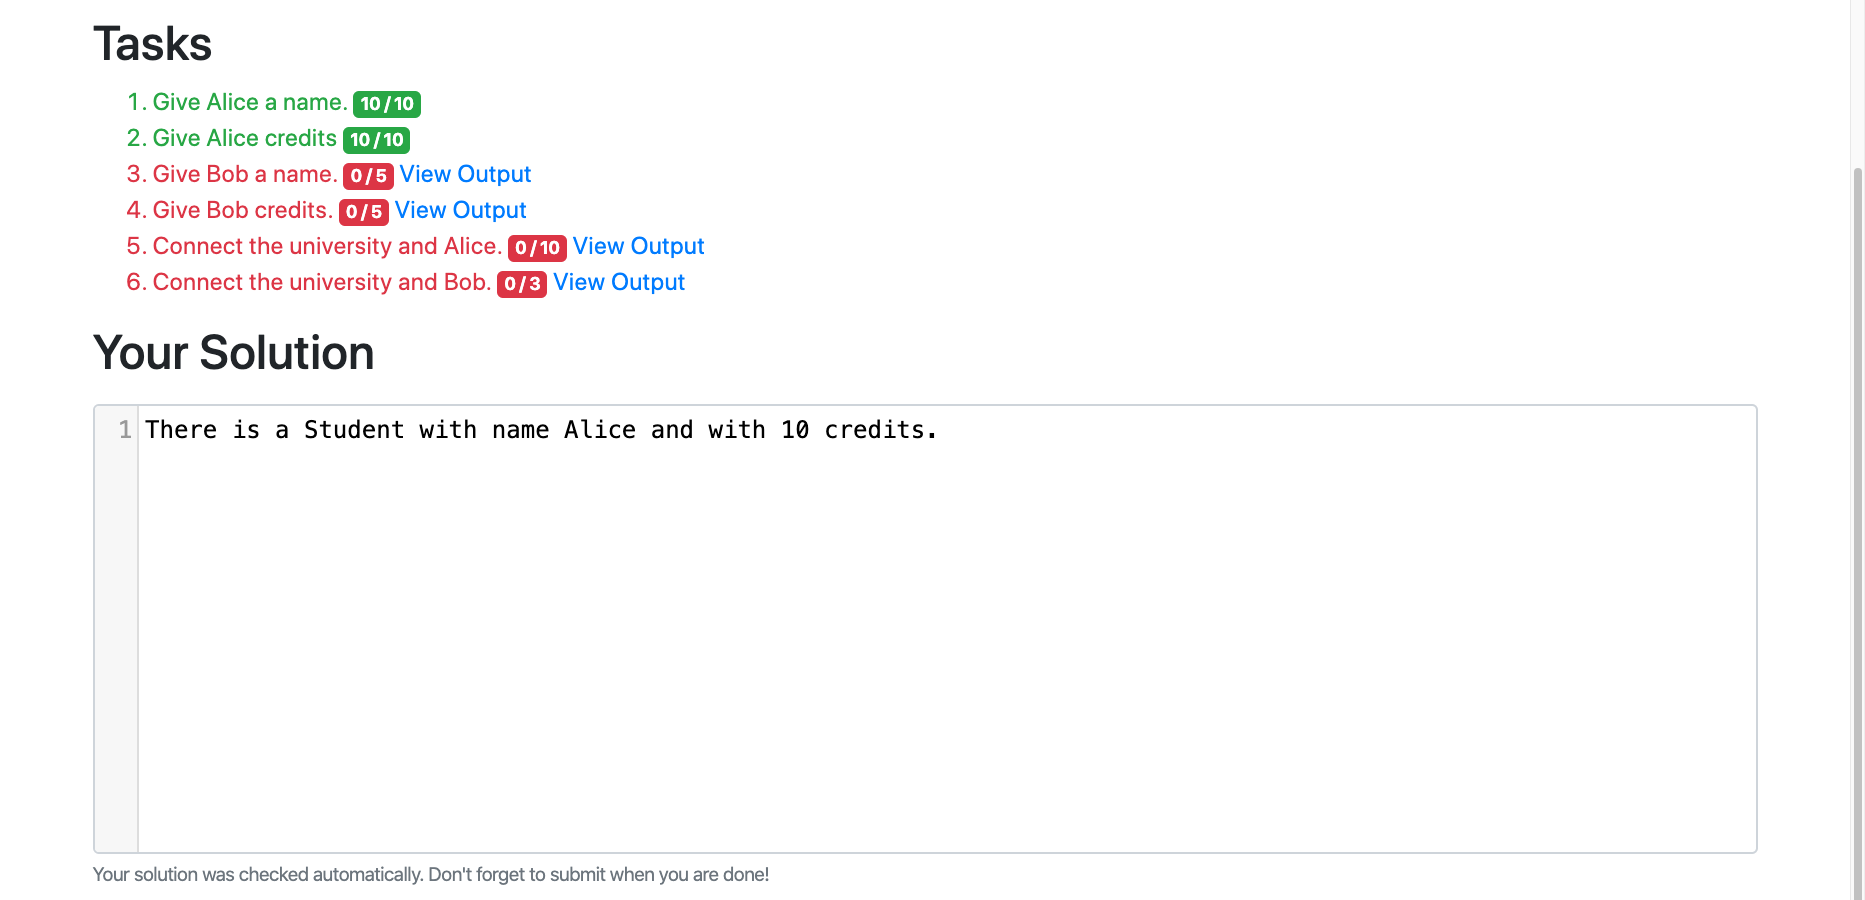
\includegraphics[width=\textwidth]{chapter/fulib.org/img/solve-tasks.png}
    \caption{Erfüllte und unerfüllte Tasks}
    \label{fig:solve-tasks}
\end{figure}

Um die Lösung abzugeben, muss der Studierende zunächst Namen, Matrikelnummer und E-Mail-Adresse angeben.
Besonders die Matrikelnummer dient später zur Identifizierung.
Daraufhin kann mit ``Submit'' die Lösung eingereicht werden.
Dies öffnet das in Abbildung~\ref{fig:solution-submitted} dargestellte Fenster.

\begin{figure}
    \centering
    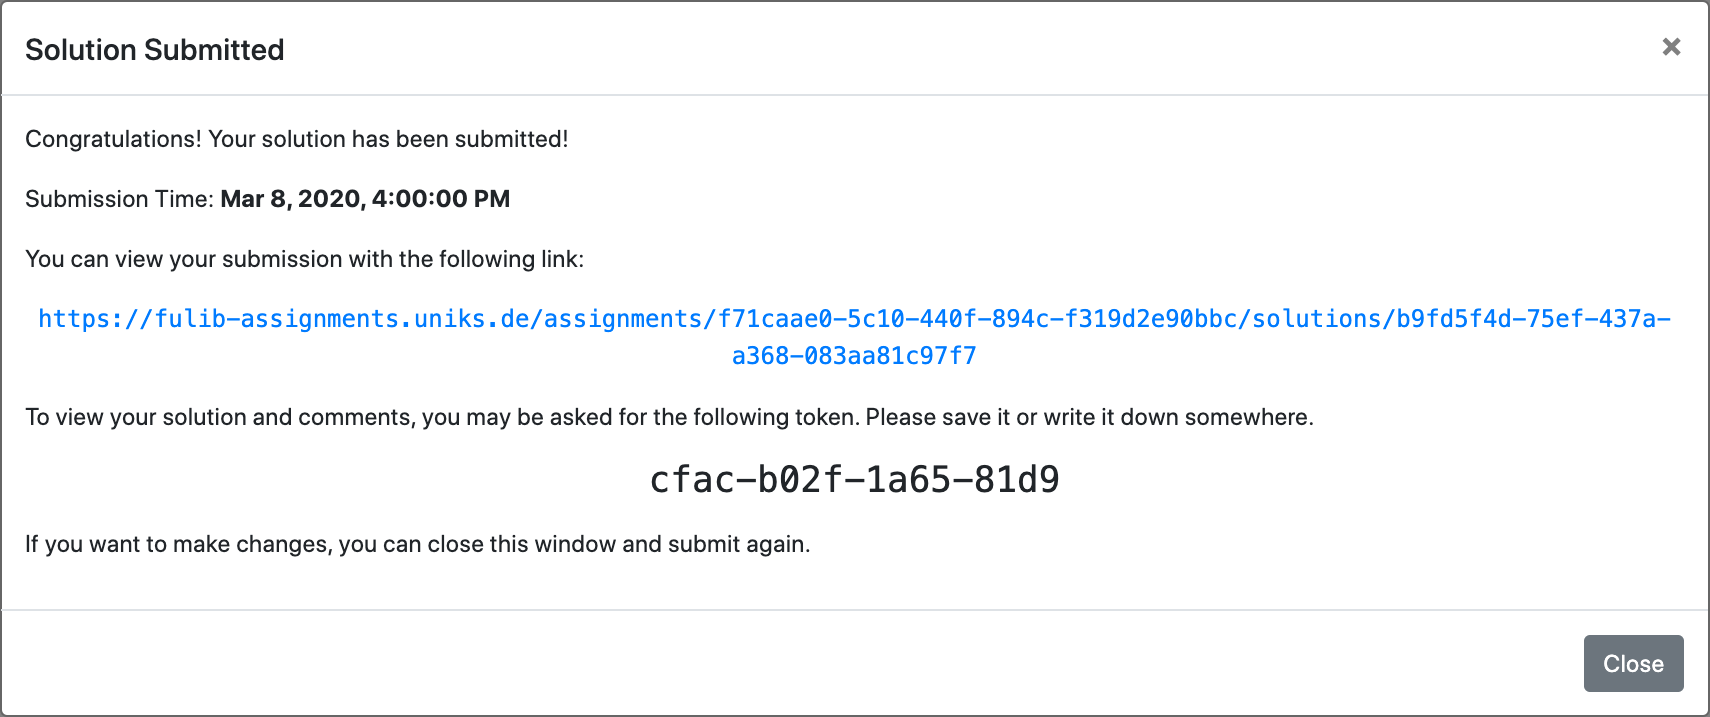
\includegraphics[width=\textwidth]{chapter/fulib.org/img/solution-submitted.png}
    \caption{Fenster nach Einreichen einer Lösung}
    \label{fig:solution-submitted}
\end{figure}

Auch für Lösungen wird ein Link und ein Token generiert.
Der Link dient dazu, die Lösung sowie deren Bewertung später einsehen zu können.
Dies ist aus Sicherheitsgründen nur mit dem Token möglich.
Zwar wird dieses im Browser gespeichert, beim Öffnen der Lösungsseite mit einem anderen Gerät muss es jedoch eingegeben werden.

Nach der Abgabe kann die Lösung weiter bearbeitet werden.
Dazu muss lediglich das Bestätigungsfenster geschlossen werden.
Durch erneutes Betätigen von ``Submit'' wird die neue Lösung eingereicht;
die alte Abgabe bleibt jedoch unverändert und weiterhin einsehbar.
Auch bei einem späteren Besuch der Seite bleiben sämtliche Eingaben bestehen, da sie lokal im Browser gespeichert werden.
Dadurch kann an einer angefangen Lösung bedenkenlos später weitergearbeitet werden,
ohne sie zwischenzeitlich einreichen zu müssen.

Studierende können ihre abgegebenen Lösungen einsehen, indem sie die Seite unter Assignments \textrightarrow{} My Solutions im Footer öffnen.
Dort finden sie nach Assignment gruppiert sämtliche eingereichte Versionen.
Abbildung~\ref{fig:my-solutions} zeigt, wie dies aussehen kann.
Der Button ``Edit'' erlaubt die Bearbeitung und erneute Abgabe einer Lösung.
Genauer öffnet er nur die Bearbeitungsseite des Assignments,
wo die zuletzt im Browser gespeicherte Lösung angezeigt wird.
Diese kann u.U.\ von der zuletzt abgegebenen Version abweichen,
wenn Änderungen vorgenommen aber nicht eingereicht wurden.

\begin{figure}
    \centering
    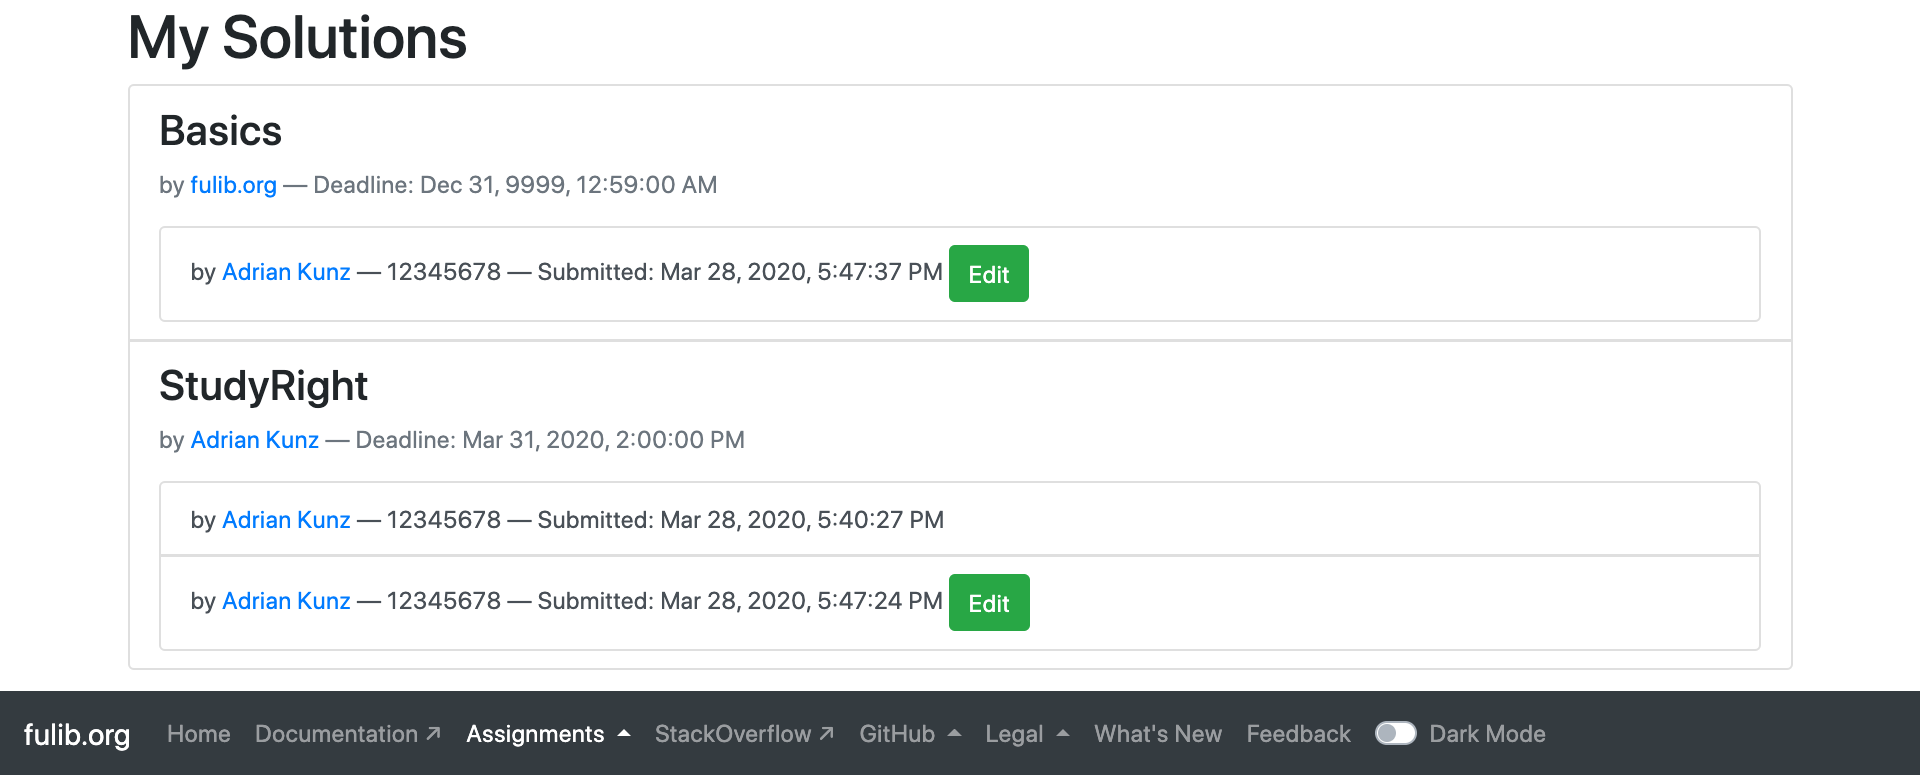
\includegraphics[width=\textwidth]{chapter/fulib.org/img/my-solutions.png}
    \caption{Liste der abgegebenen Lösungen}
    \label{fig:my-solutions}
\end{figure}

\subsection{Korrigieren}\label{subsec:correcting}

Einstiegspunkt für die Korrektur ist die Seite, auf der abgegen Lösungen für ein Assignment einsehbar sind.
Diese ist unter dem zweiten Link erreichbar, der nach Anlegen eines Assignments erzeugt wurde.
Der Kursleiter kann diesen an die Korrekteure zusammen mit dem Token weiterleiten.
Beim ersten Besuch des Links muss letzteres angebeben werden, um die Lösungen anzuzeigen.
Daraufhin zeigt sich die Tabelle mit Lösungen, die in Abbildung~\ref{fig:solution-table} zu sehen ist.

\begin{figure}
    \centering
    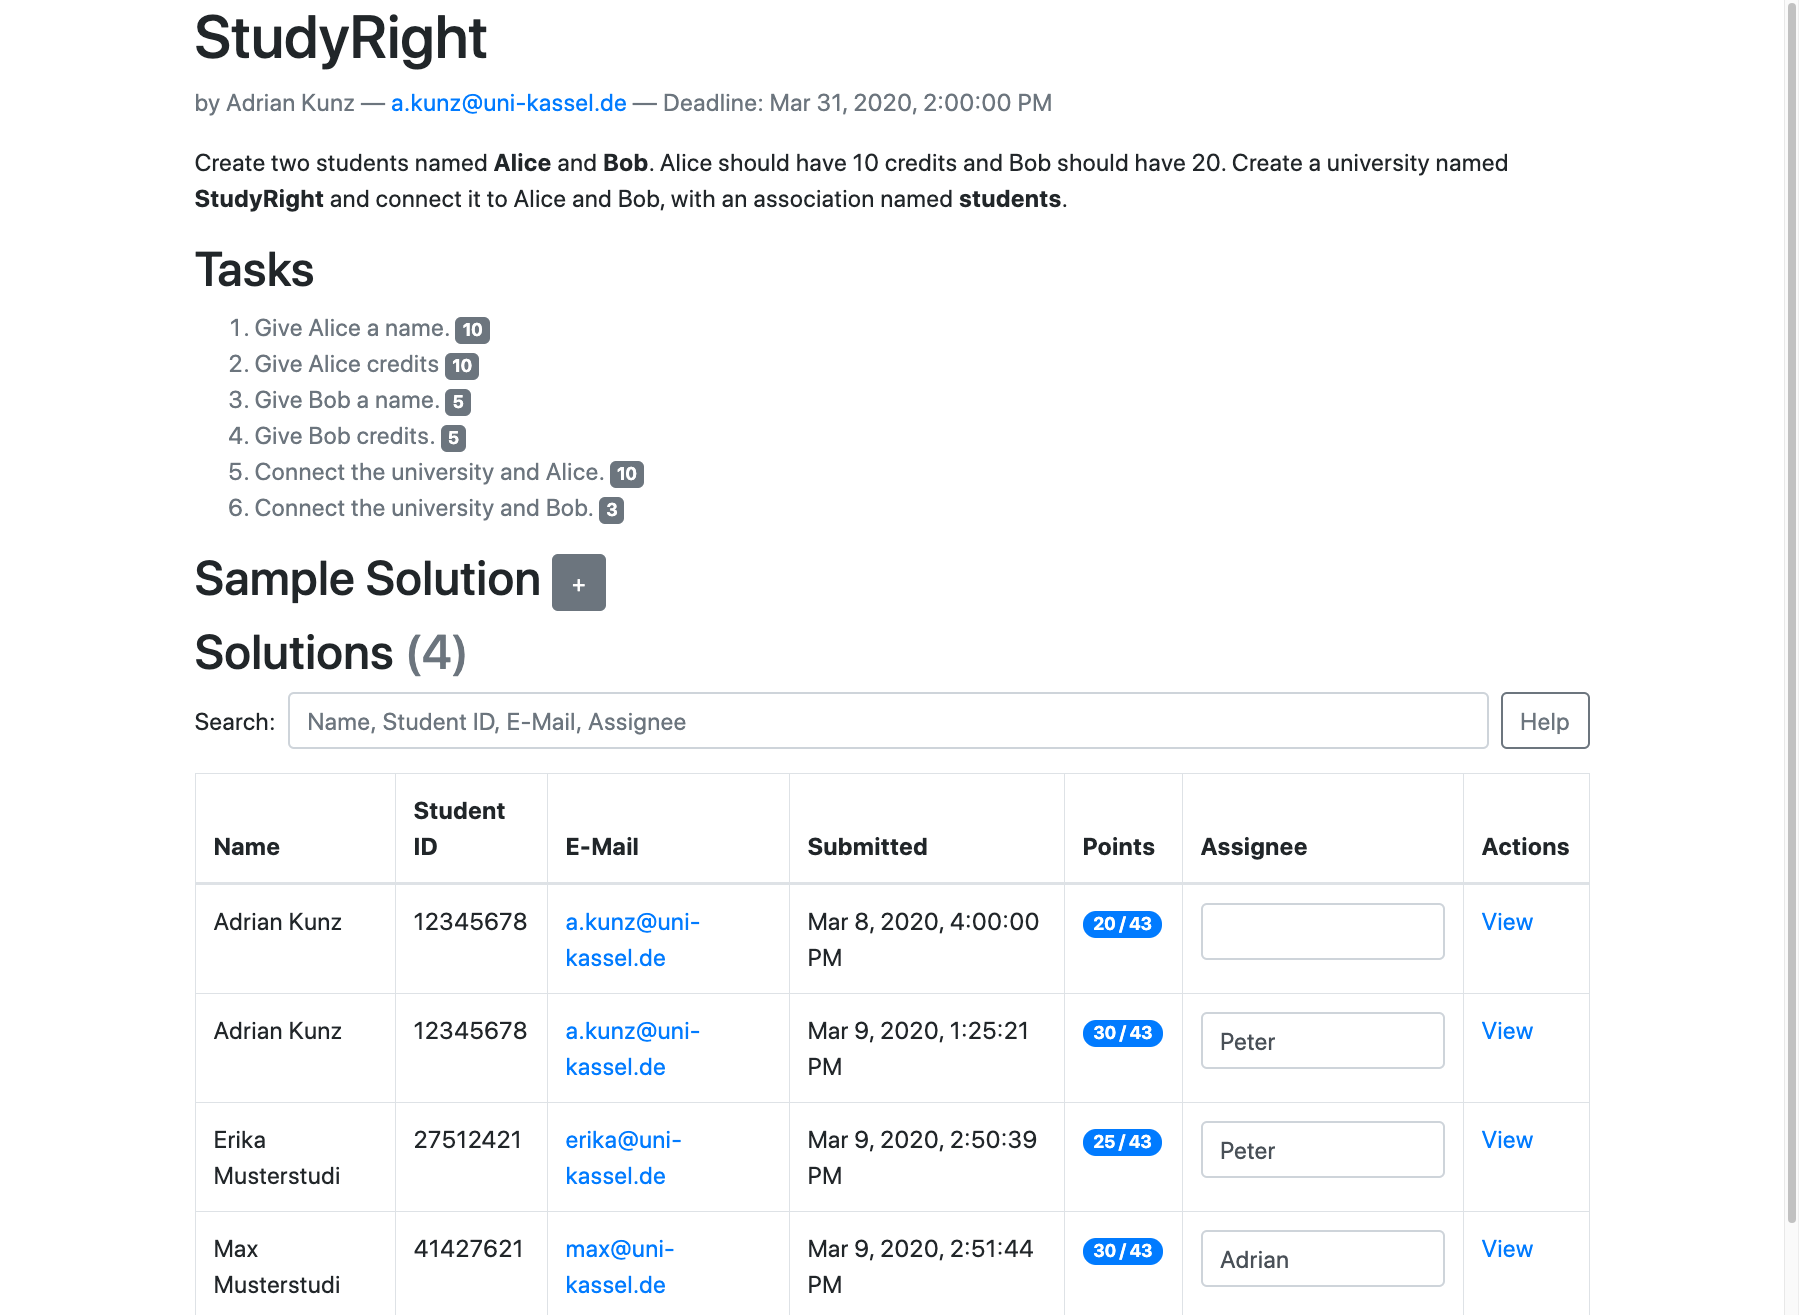
\includegraphics[width=\textwidth]{chapter/fulib.org/img/solution-table.png}
    \caption{Tabelle der eingereichten Lösungen für ein Assignment}
    \label{fig:solution-table}
\end{figure}

Über der Tabelle befindet sich eine Übersicht der Aufgabenstellung, inklusive Eckdaten, Beschreibung, Tasks und eventueller Musterlösung.
Dies vereinfacht die Korrektur, da keine separate Seite geöffnet werden muss, um diese einzusehen.
Das Suchfeld erlaubt es, die angezeigten Lösungen einzuschränken.
Dies ist sowohl als Freitextsuche über alle Spalten als auch für bestimmte Spalten möglich.
So lässt sich beispielsweise mit \code{assignee:Peter} nach allen Lösungen suchen, die dem Korrekteur \code{Peter} zugewiesen sind.
Die Zuweisung erfolg durch Ändern des Eingabefelds unter ``Assignee'' und wird sofort übernommen.
I.d.R.\ kann der Kursleiter diese Zuordnung durchführen, woraufhin die Korrekteure nach den ihnen zugewiesenen Lösungen suchen können.

Die Tabelle gibt zunächst eine Übersicht über die Randangaben der Lösung.
Dazu gehören neben den Angaben zum Studierenden auch das Abgabedatum sowie die erreichte Punktzahl.
Nach der Deadline abgegebene Lösungen werden rot hervorgehoben.
Durch Klick auf ``View'' gelangt man zur Detailseite der Lösung, die in Abbildung~\ref{fig:solution} dargestellt ist.

\begin{figure}
    \centering
    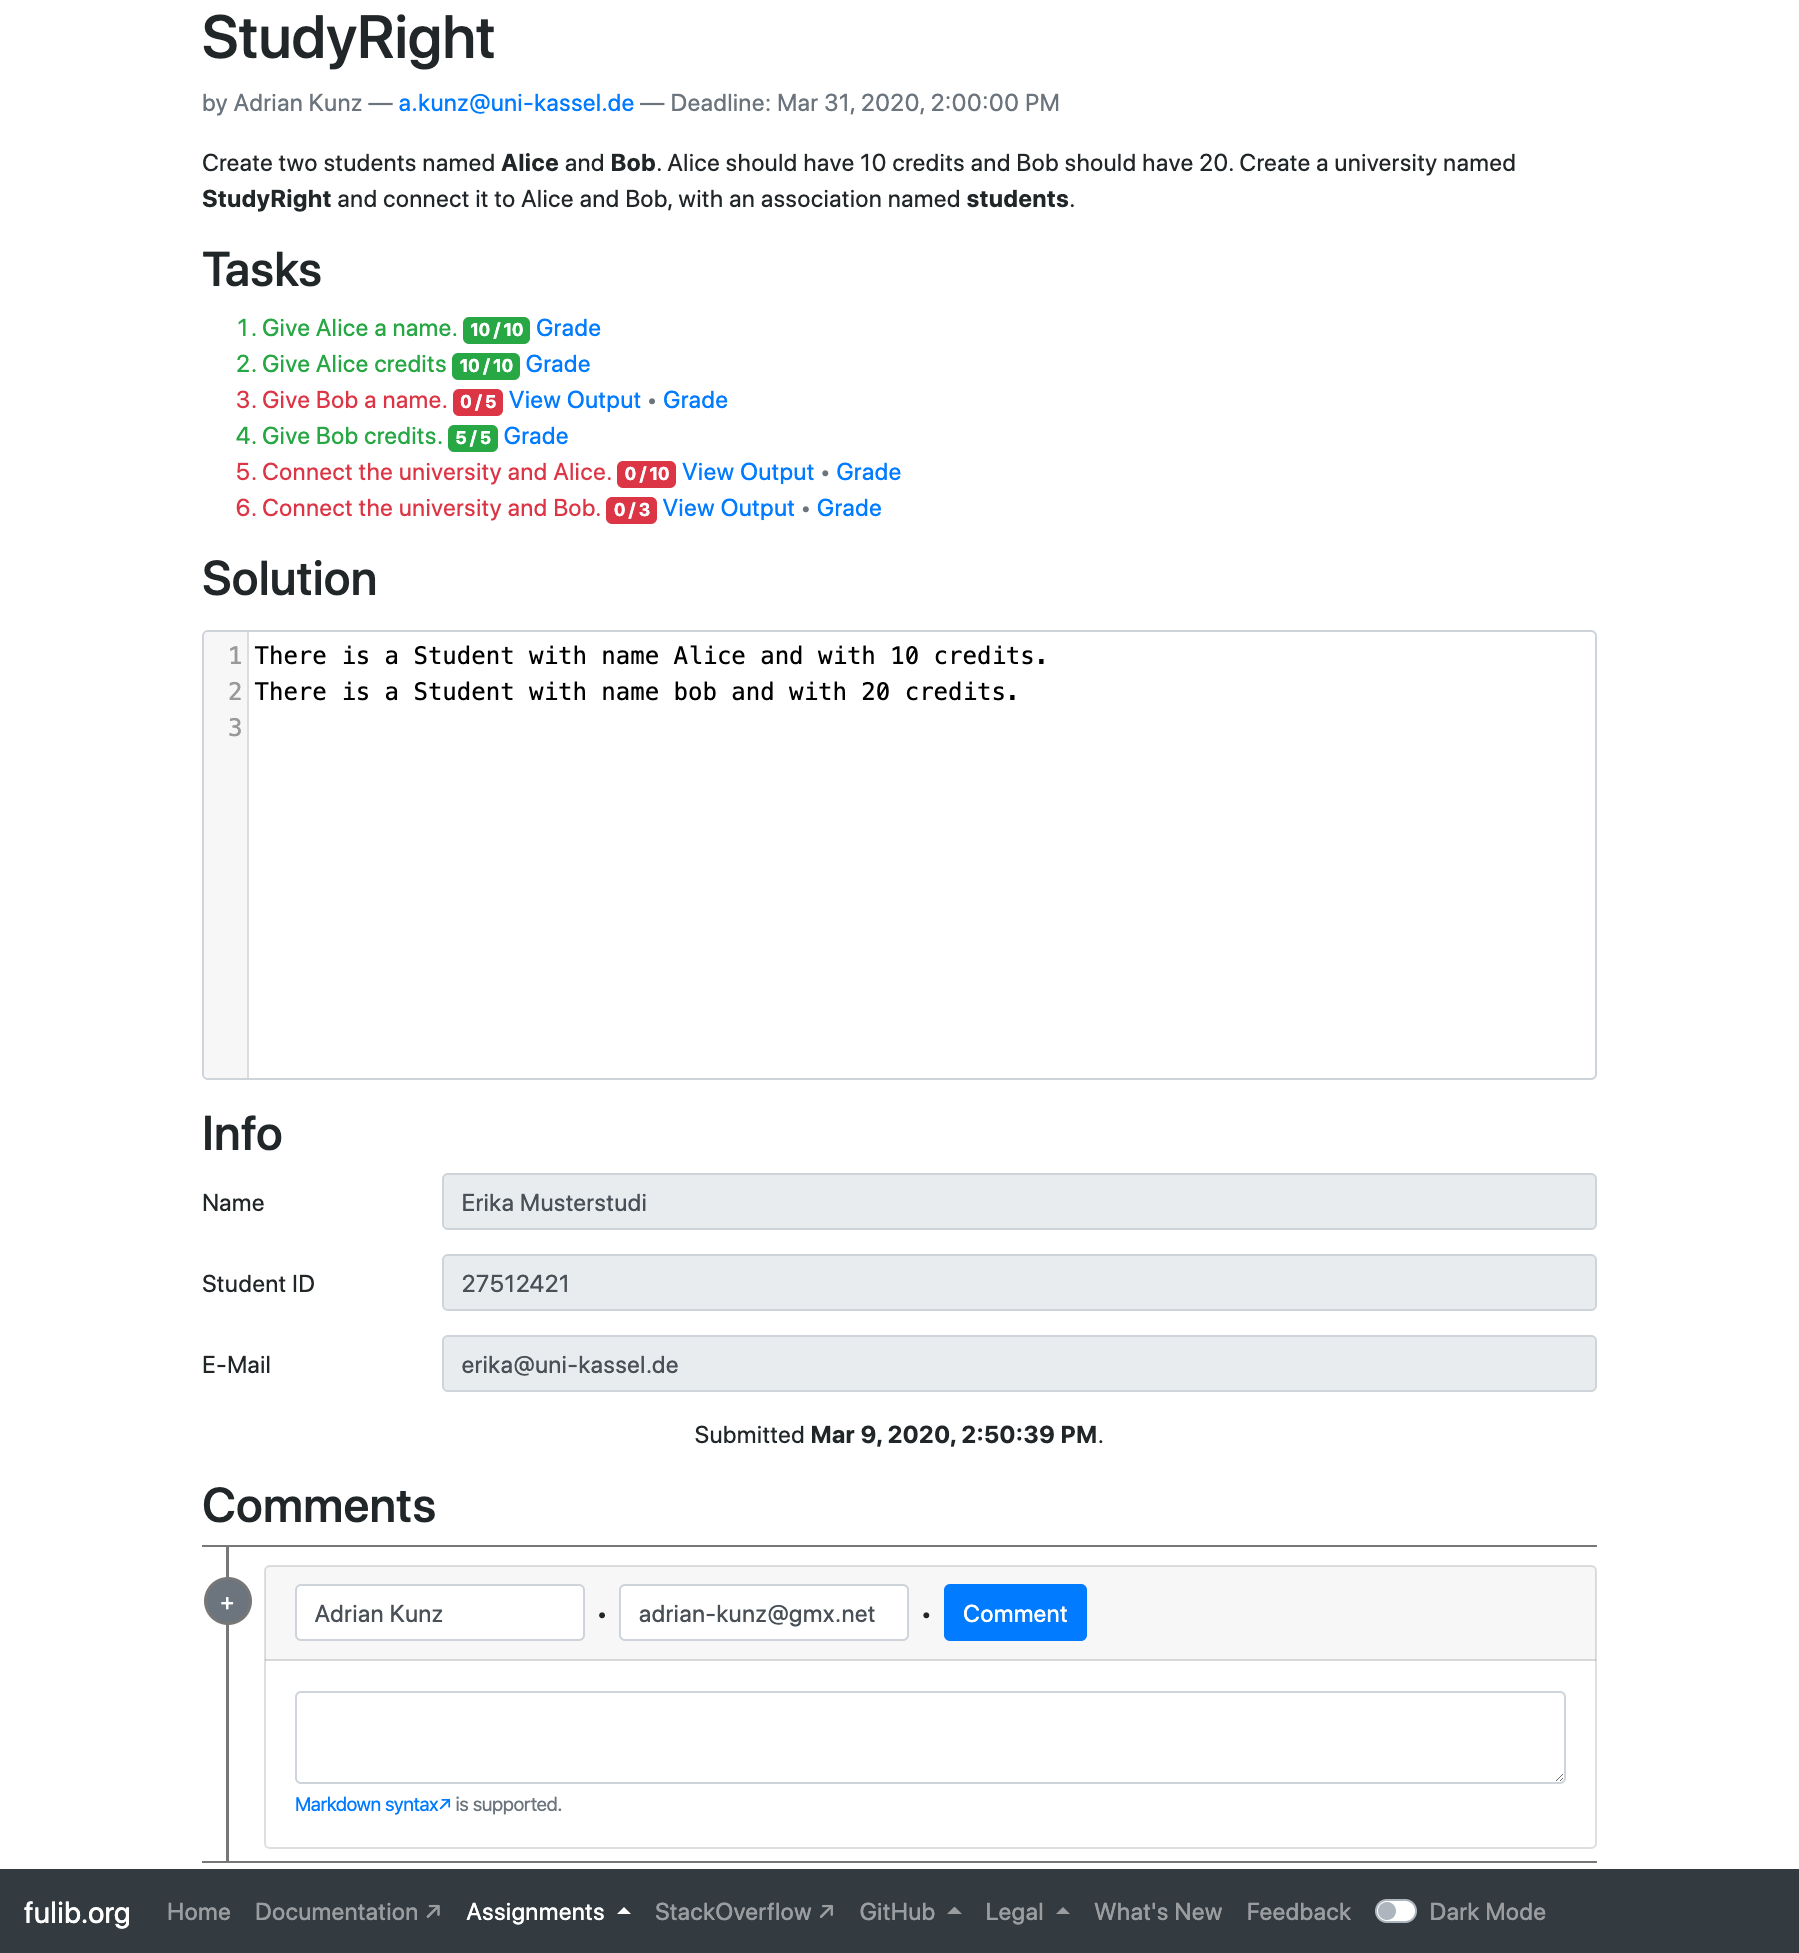
\includegraphics[width=\textwidth]{chapter/fulib.org/img/solution.png}
    \caption{Ansicht einer abgegebenen Lösung}
    \label{fig:solution}
\end{figure}

Hier wird erneut die Aufgabenstellung angezeigt;
die Task-Liste zeigt hier wie bei der Bearbeitung die erreichte Punktzahl.
Mit ``Grade'' kann der Korrekteur darin die Bewertung anpassen.
Dabei muss die zu vergebene Punktzahl, ein kurzer Kommentar und der eigene Name angegeben werden.
In der Historie werden alle Änderungen der Bewertung aufgelistet.
Auch Studierende können diese einsehen, jedoch nicht verändern, da dafür das Token des Assignments benötigt wird.
Abbildung~\ref{fig:grade-popover} zeigt das Fenster der Bewertung eines Tasks.
Aufgrund der Vergabe von Teilpunkten wurde der entsprechende Task gelb, was bei der automatischen Bewertung nicht möglich ist.

\begin{figure}
    \centering
    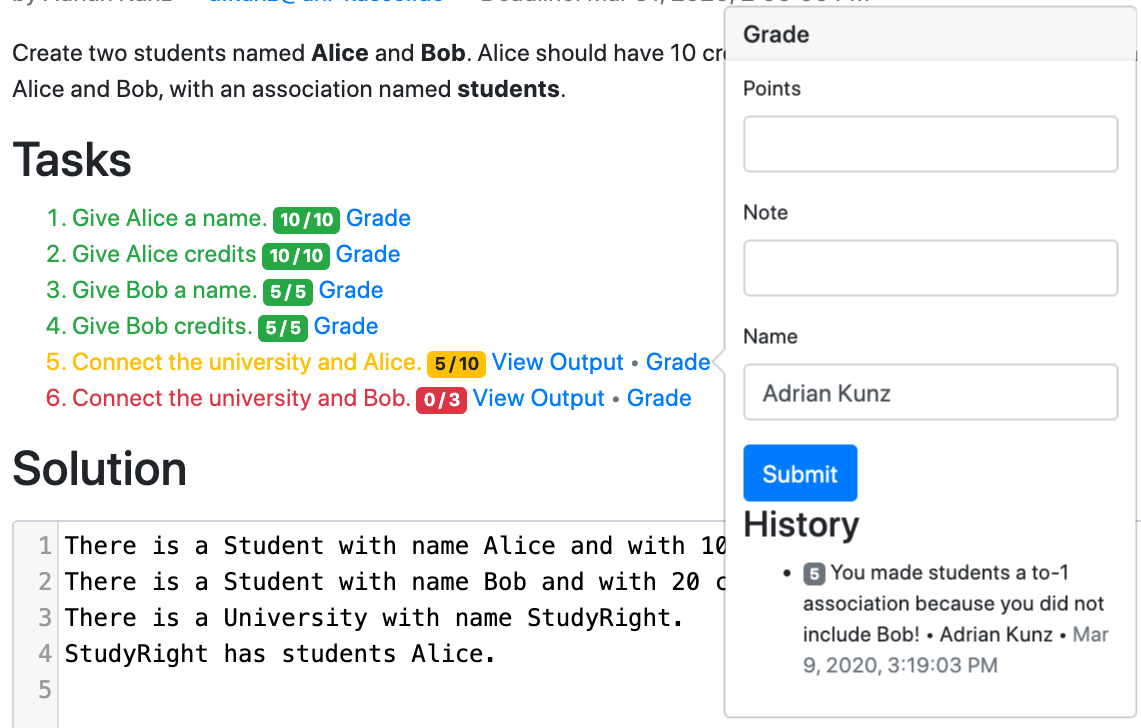
\includegraphics[width=0.5\textwidth]{chapter/fulib.org/img/grade-popover.png}
    \caption{Fenster zur Bewertung eines Tasks}
    \label{fig:grade-popover}
\end{figure}

Am unteren Ende der Seite befindet sich der Kommentarbereich.
Hier können Studierende und Korrekteure Fragen, Antworten und Anmerkungen zur Bewertung hinterlassen.
Hat man das Token des Assignmenst und erstellt ein Kommentar,
wird dieses mit einem Häkchen hinter dem Namen hervorgehoben.
Dies verhindert, dass Studierende durch Angabe des Namens des Kursleiters oder eines Korrekteurs diese imitieren können.

\subsection{Kurse}\label{subsec:courses}

Kurse sind Sammlungen von Assignments, die eine feste Reihenfolge vorgeben.
Sie ermöglichen die Vergabe von mehreren Aufgabenstellungen, die inhaltlich zusammen gehören und aufeinander aufbauen können.
So ist es beispielsweise möglich, einen unbeaufsichtigten, von einer Vorlesung unabhängigen Kurs zu erstellen, mit dem die Scenario-Sprache erlernt werden kann.
Interessierte können diesen aufrufen und selbstständig Assignments bearbeiten, die nicht von Korrekteuren bewertet werden.

Kurse werden erstellt, indem im Footer Assignments \textrightarrow{} Create Course ausgewählt wird.
Dies öffnet die in Abbildung~\ref{fig:create-course} gezeigte Seite.

\begin{figure}
    \centering
    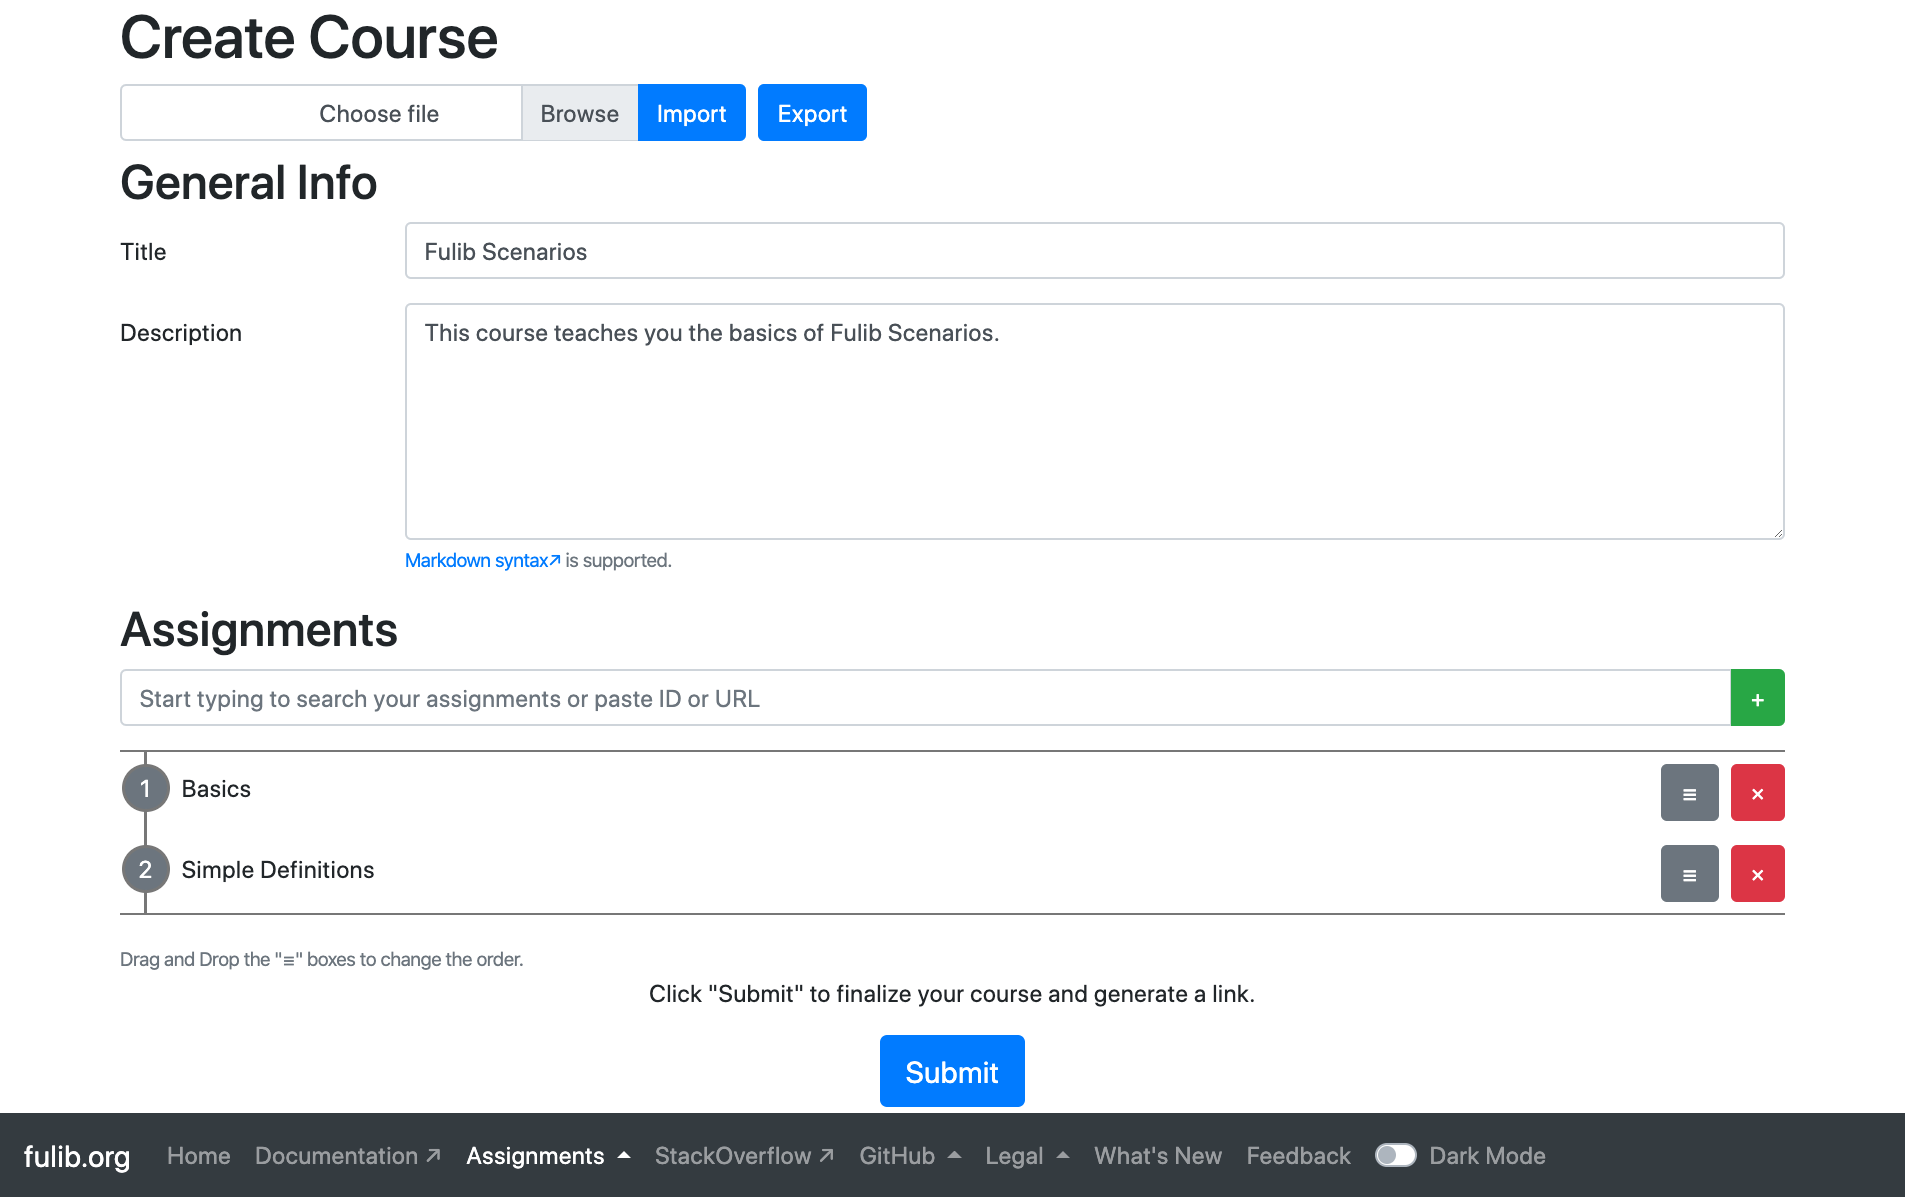
\includegraphics[width=\textwidth]{chapter/fulib.org/img/create-course.png}
    \caption{Formular zum Erstellen eines Kurses}
    \label{fig:create-course}
\end{figure}

Ein Kurs benötigt neben den zugehörigen Assignments einen Titel und eine Beschreibung.
Assignments müssen im Vorhinein mit dem in Unterabschnitt~\ref{subsec:creation} erläuterten Formular erstellt werden.
Diese lassen sich dann mit dem dafür vorgesehenen Feld dem Kurs hinzufügen.
Alternativ können beliebige Assignments von anderen Autoren eingebunden werden,
solange der zugehörige Link bekannt ist.
Die dabei entstehenden Liste erlaubt ferner das Umordnen sowie Entfernen der hinzugefügten Assignments.
Dafür werden die gleiche Steuerelemente wie bei der Task-Liste beim Anlegen eines Assignments verwendet.
Zum Erstellen genügt nach Ausfüllen des Formulars ein Klick auf den Button ``Submit''.
Dabei wird für den Kurs ein Link generiert, unter dem er abrufbar ist.
Abbildung~\ref{fig:course-view} zeigt die Seite, die damit aufgerufen wird.

\begin{figure}
    \centering
    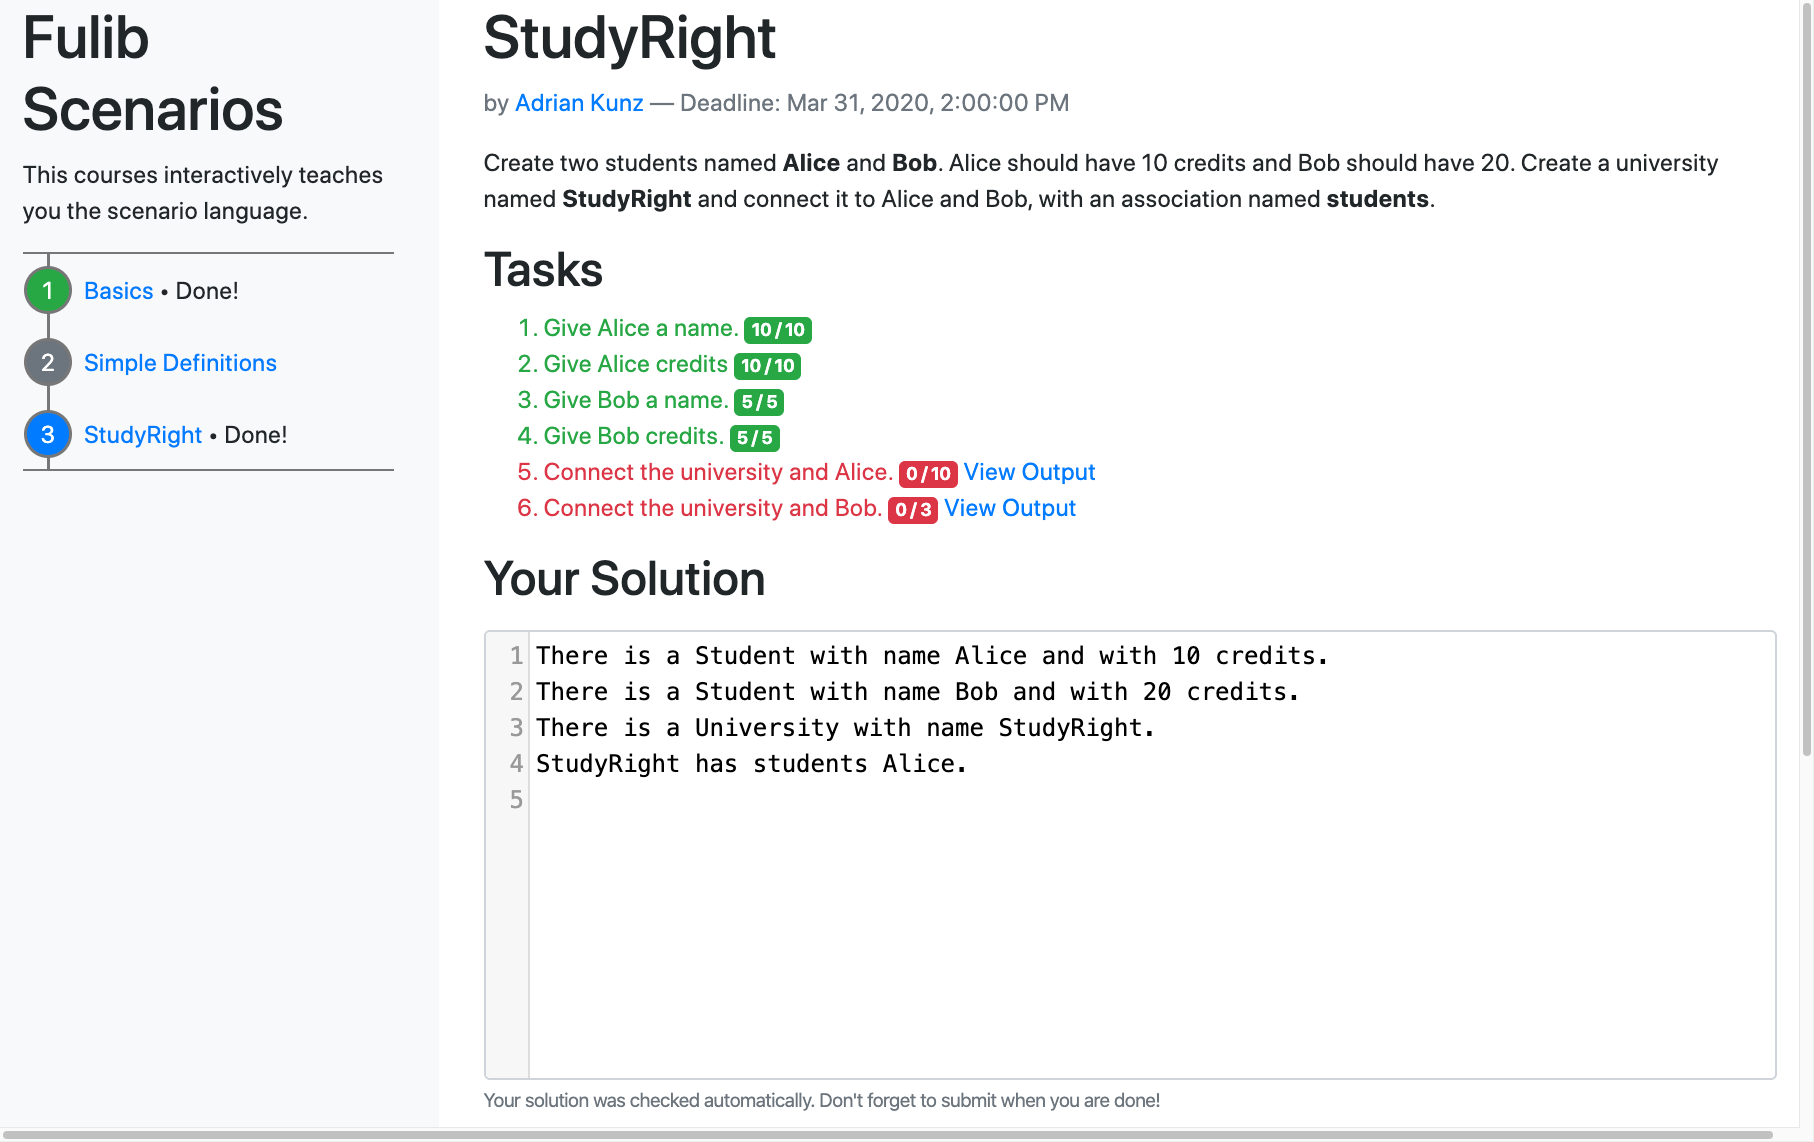
\includegraphics[width=\textwidth]{chapter/fulib.org/img/course-view.png}
    \caption{Kurs-Ansicht}
    \label{fig:course-view}
\end{figure}

Die Bearbeitung eines Assignments in einem Kurs unterscheidet sich nur geringfügig von der eines alleinstehenden Assignments.
Hinzu kommt die Seitenleiste am linken Bildschirmrand, die Titel, Beschreibung und Verlauf des Kurses anzeigt.
Darin werden das aktuell angezeigte sowie bereits bearbeitete Assignments hervorgehoben.
Die Assignments eines Kurses können in beliebiger Reihenfolge bearbeitet werden.
Grund dafür ist, dass sie auch außerhalb des Kurses beliebig abruf- und bearbeitbar sind.
I.d.R.\ ist es jedoch sinnvoll, sich an den vorgegebene Ablauf zu halten.
Bearbeitet man ein Assignment als Teil eines Kurses und reicht eine Lösung ein, verändert sich das Bestätigungsfenster der Abgabe.
In diesem kommt ein Button hinzu, der das Fortschreiten zum nächsten Assignment im Kurs erlaubt.

\todo{
FulibScenarios-Kurs
}
